% Created 2016-09-13 Tue 15:40
\documentclass{beamer}
\usepackage{fixltx2e}
\usepackage{graphicx}
\usepackage{longtable}
\usepackage{float}
\usepackage{wrapfig}
\usepackage{soul}
\usepackage{textcomp}
\usepackage{marvosym}
\usepackage{wasysym}
\usepackage{latexsym}
\usepackage{amssymb}
\usepackage{hyperref}
\tolerance=1000
\usepackage{etex}
\usepackage{amsmath}
\usepackage{pgfplots}
\usepackage{tikz}
\usepackage[europeanresistors,americaninductors]{circuitikz}
\usepackage{colortbl}
\usepackage{yfonts}
\usetikzlibrary{shapes,arrows}
\usetikzlibrary{positioning}
\usetikzlibrary{arrows,shapes}
\usetikzlibrary{intersections}
\usetikzlibrary{calc,patterns,decorations.pathmorphing,decorations.markings}
\usepackage[BoldFont,SlantFont,CJKchecksingle]{xeCJK}
\setCJKmainfont[BoldFont=Evermore Hei]{Evermore Kai}
\setCJKmonofont{Evermore Kai}
\xeCJKsetup{CJKglue=\hspace{0pt plus .08 \baselineskip }}
\mode<beamer>{\usetheme{JuanLesPins}}
\mode<beamer>{\usetheme{Frankfurt}}
\mode<beamer>{\usecolortheme{dove}}
\usepackage{underscore}
\AtBeginSection[]{\begin{frame}<beamer>\frametitle{Topic}\tableofcontents[currentsection]\end{frame}}
\setbeamercovered{transparent}
\providecommand{\alert}[1]{\textbf{#1}}

\title{人工神经网络}
\author{}
\date{}
\hypersetup{
  pdfkeywords={},
  pdfsubject={},
  pdfcreator={Emacs Org-mode version 7.9.3f}}

\begin{document}

\maketitle

\begin{frame}
\frametitle{Outline}
\setcounter{tocdepth}{3}
\tableofcontents
\end{frame}












\section{简介}
\label{sec-1}
\begin{frame}
\frametitle{人工神经网络(Artificial Neural Networks——ANNs)}
\label{sec-1-1}


\begin{itemize}
\item 人工神经网络(Artificial Neural Networks——ANNs)提供了一种普遍而且实用的方法,来从样例中学习值为实数、离散或向量的函数。
\item 反向传播(BackPropagation)算法使用梯度下降来调节网络参数以最佳拟合由输入-输出对组成的训练集合。
\item ANN学习对于训练数据中的错误鲁棒性很好,且已经成功地应用到很多领域,例如
\begin{itemize}
\item 视觉场景分析(interpreting visual scenes)
\item 语音识别
\item 机器人控制
\item \ldots{}...
\end{itemize}
\end{itemize}
\end{frame}
\begin{frame}[fragile]
\frametitle{示例}
\label{sec-1-2}


\begin{itemize}
\item Pomerleau(1993)的 ALVINN (Autonomous Land Vehicle In a Neural Network)系统是ANN学习的一个典型实例,

\begin{verbatim}
http://ftp.utcluj.ro/pub/docs/imaging/
Autonomous_driving/Articole%20sortate/
CThorpe/ALVINN%20Project%20Home%20Page.htm
\end{verbatim}
\item 这个系统使用一个学习到的ANN以正常的速度在高速公路上驾驶汽车。
\begin{itemize}
\item ANN的输入是一个30x32像素的网格,像素的亮度来自一个安装在车辆上的前向摄像机。
\item ANN的输出是车辆行进的方向。
\item 这个ANN通过观察人类驾驶时的操纵命令进行训练,训练过程大约5分钟。
\end{itemize}
\item ALVINN用学习到的网络在高速公路上以70英里时速成功地驾驶了90英里(在分行公路的左车道行驶,同时有其他车辆)。
\end{itemize}
\end{frame}
\begin{frame}
\frametitle{示例(ALVINN系统)}
\label{sec-1-3}

\center
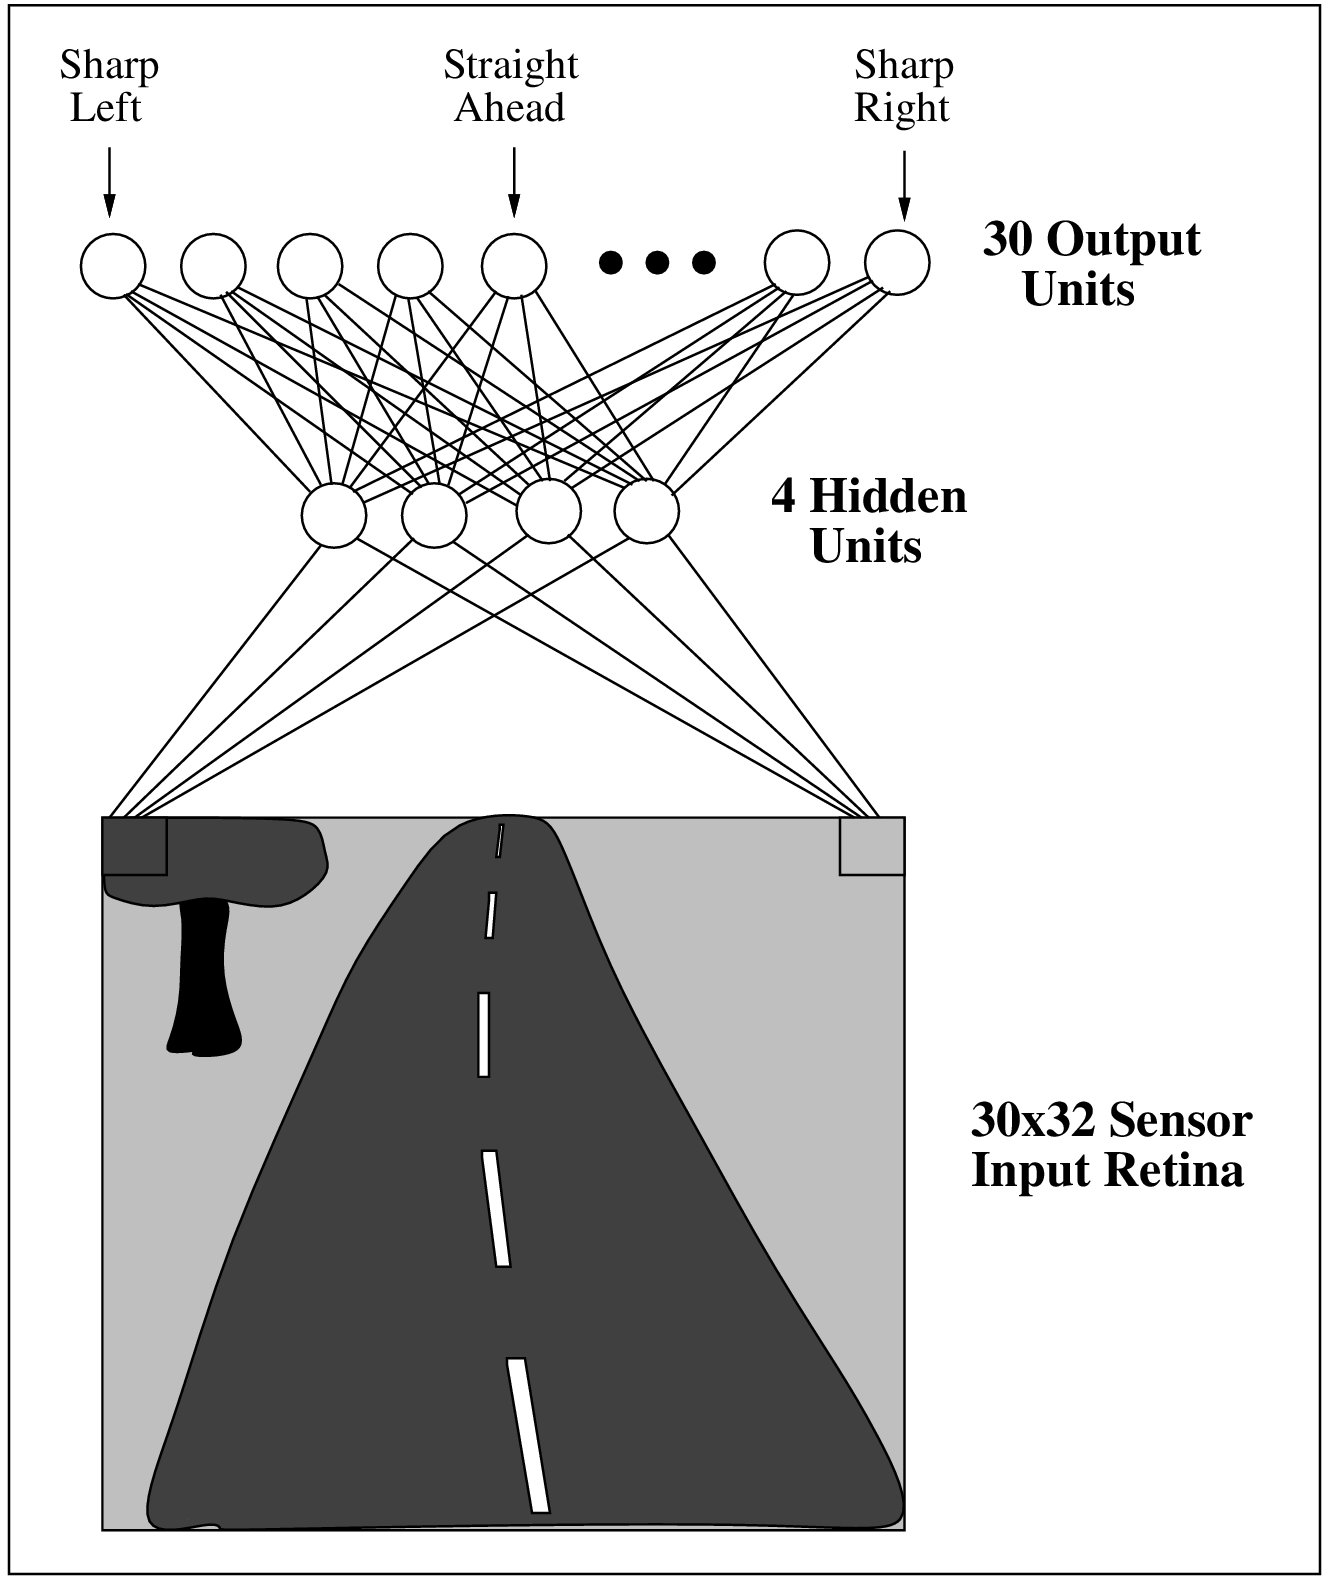
\includegraphics[width=0.6\textwidth]{./image/alvinn1.png}
\end{frame}
\begin{frame}
\frametitle{示例(ALVINN原理)}
\label{sec-1-4}

\center
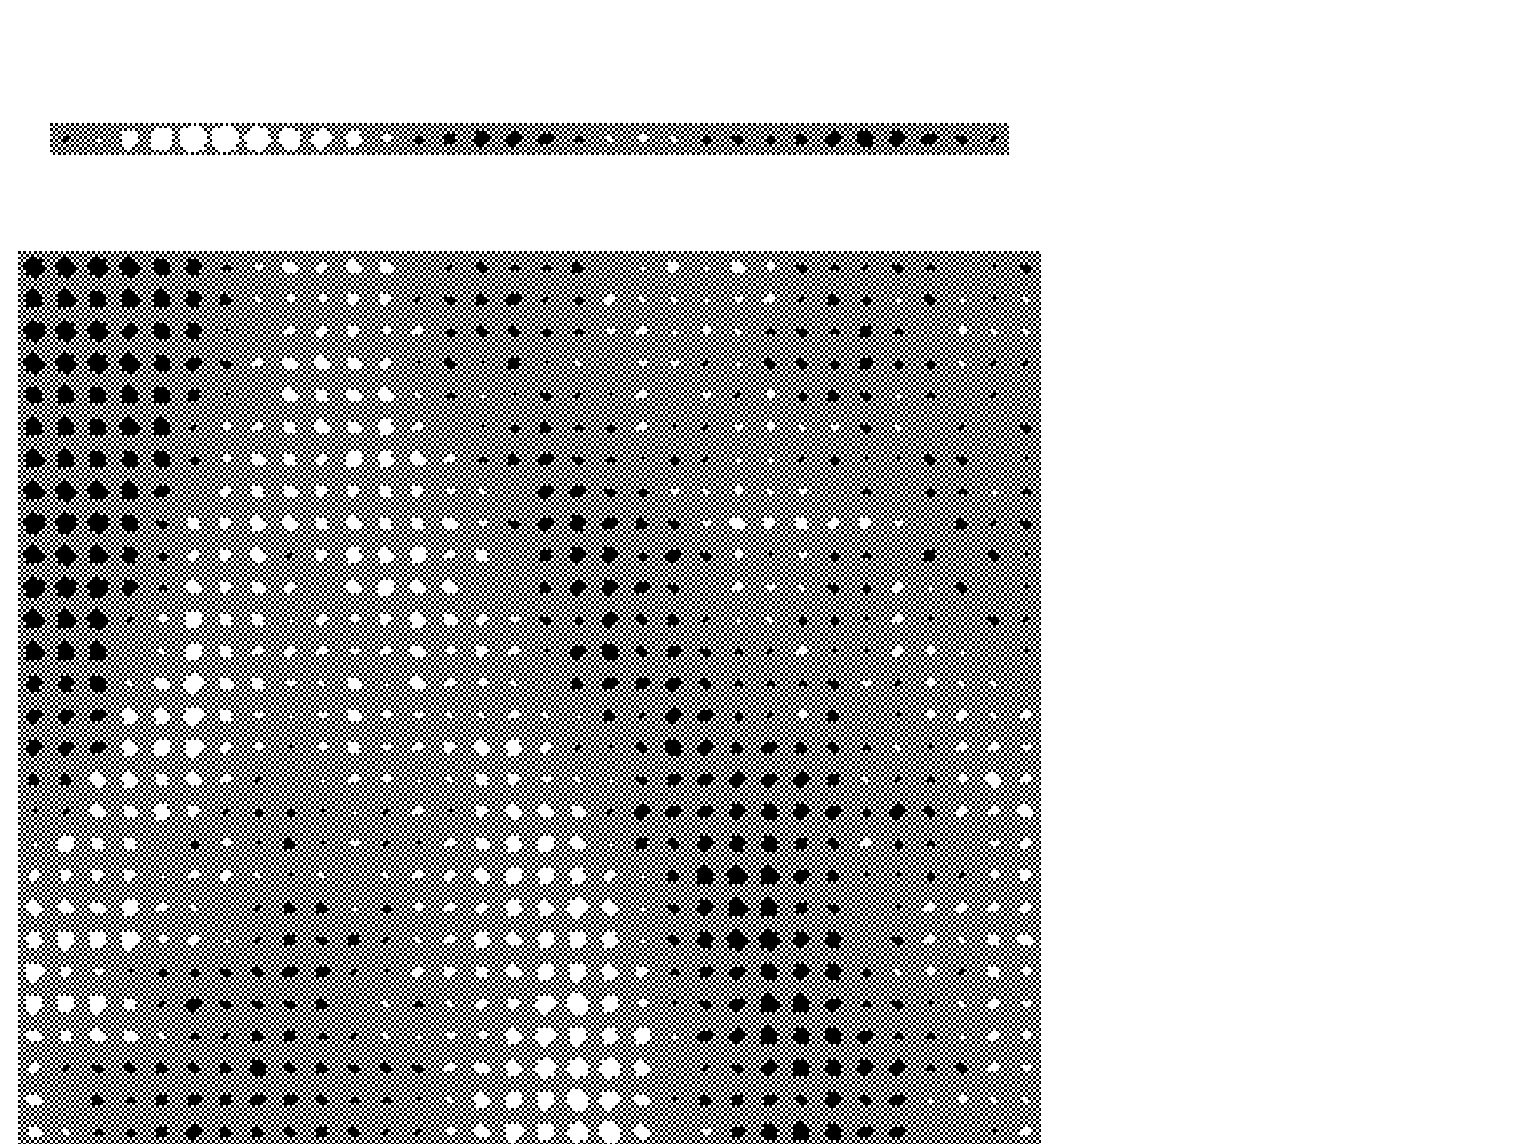
\includegraphics[width=0.6\textwidth]{./image/alvinn2.png}
\end{frame}
\begin{frame}
\frametitle{示例(隐藏单元权值)}
\label{sec-1-5}

\center
\includegraphics[width=0.6\textwidth]{./image/alvinn3.png}
\end{frame}
\begin{frame}
\frametitle{人工神经网络适用问题}
\label{sec-1-6}


\begin{itemize}
\item 实例是用很多“属性-值”对表示的。
\begin{itemize}
\item 要学习的目标函数是定义在可以用向量描述的实例之上的,向量由预先定义的特征组成,
\begin{itemize}
\item 例如ALVINN例子中的像素值。
\end{itemize}
\item 这些输入属性之间可以高度相关,也可以相互独立。
\item 输入值可以是任何实数。
\end{itemize}
\item 目标函数的输出可能是离散值、实数值或者由若干实数属性或离散属性组成的向量。
\begin{itemize}
\item 例如,
\begin{itemize}
\item 在ALVINN系统中输出的是30个属性的向量,每一个分量对应一个建议的驾驶方向。
\item 每个输出值是0和1之间的某个实数,对应于在预测相应驾驶方向时的置信度(confidence)。
\item 我们也可以训练一个单一网络,同时输出行驶方向和建议的加速度,这只要简单地把编码这两种输出预测的向量连接在一起就可以了。
\end{itemize}
\end{itemize}
\end{itemize}
\end{frame}
\begin{frame}
\frametitle{人工神经网络适用问题(续)}
\label{sec-1-7}

\begin{itemize}
\item 训练数据可能包含错误。
\begin{itemize}
\item ANN学习算法对于训练数据中的错误有非常好的鲁棒性。
\end{itemize}
\item 可容忍长时间的训练。
\begin{itemize}
\item 网络训练算法通常比像决策树学习这样的算法需要更长的训练时间。
\begin{itemize}
\item 训练时间可能从几秒钟到几小时,这要看网络中权值的数量、要考虑的训练实例的数量、以及不同学习算法参数的设置等因素。
\end{itemize}
\end{itemize}
\item 可能需要快速求出目标函数值。
\begin{itemize}
\item 尽管ANN的学习时间相对较长,但对学习到的网络求值,以便把网络应用到后续的实例,通常是非常快速的。
\begin{itemize}
\item 例如,ALVINN在车辆向前行驶时,每秒应用它的神经网络若干次,以不断地更新驾驶方向。
\end{itemize}
\end{itemize}
\item 人类能否理解学到的目标函数是不重要的。
\begin{itemize}
\item 神经网络方法学习到的权值经常是人类难以解释的。
\item 学到的神经网络比学到的规则难于传达给人类。
\end{itemize}
\end{itemize}
\end{frame}
\section{感知器}
\label{sec-2}
\begin{frame}
\frametitle{感知器}
\label{sec-2-1}

\includegraphics[width=0.6\textwidth]{./image/perceptron.png}

\[o(x_{1}, \ldots, x_{n}) = \left\{ \begin{array}{rl}
     1 & \mbox{if $w_{0} + w_{1}x_1 + \cdots + w_n x_n > 0$}\\
     -1 & \mbox{otherwise.}  
\end{array}
\right. \]

 简化表示:

\[
o(\vec{x}) = \left\{ \begin{array}{rl}
     1 & \mbox{if $\vec{w} \cdot \vec{x} > 0$}\\
     -1 & \mbox{otherwise.}  
\end{array}
\right. 
\]
\end{frame}
\begin{frame}
\frametitle{两输入感知器的决策平面}
\label{sec-2-2}


\includegraphics[width=.9\linewidth]{./image/ann-linearly-separable.png}
\end{frame}
\begin{frame}
\frametitle{感知器训练法则(perceptron learning rule)}
\label{sec-2-3}


\[w_i \leftarrow w_i + \Delta w_i \]
where
\[ \Delta w_{i} = \eta (t - o) x_{i} \]

其中:

\begin{itemize}
\item $t=c(\vec{x})$ 是当前训练样例的目标输出
\item $o$ 是感知器的输出
\item $\eta$ 是一个正的常数称为学习速率(learning rate)
\end{itemize}
\end{frame}
\begin{frame}
\frametitle{收敛性}
\label{sec-2-4}


\begin{itemize}
\item 在有限次使用感知器训练法则后,训练过程会收敛到一个能正确分类所有训练样例的权向量,
\end{itemize}

前提:

\begin{itemize}
\item 训练样例线性可分,
\item 使用了充分小的 $\eta$ (参见Minskey \& Papert 1969)
\end{itemize}
\end{frame}
\begin{frame}
\frametitle{梯度下降和delta法则}
\label{sec-2-5}


考虑线性单元:

\[ o = w_{0} + w_{1}x_1 + \cdots + w_n x_n \]

学习使均方误差

\[ E[\vec{w}] \equiv  \frac{1}{2}\sum_{d \in D}(t_{d} - o_{d})^{2} \]

最小的  $w_{i}$ 。其中 $D$ 训练样例集合。
\end{frame}
\begin{frame}
\frametitle{误差曲面}
\label{sec-2-6}

\center
\includegraphics[width=0.6\textwidth]{./image/parabola-floor.png}
\end{frame}
\begin{frame}
\frametitle{梯度下降算法}
\label{sec-2-7}


\[ \nabla E[\vec{w}] \equiv \left[\frac{\partial E}{\partial w_{0}},
\frac{\partial E}{\partial w_{1}}, \cdots \frac{\partial E}{\partial
w_{n}}\right] \]

训练法则:

\[\Delta \vec{w} = -\eta \nabla E[\vec{w}] \]

或:

\[\Delta w_{i} = -\eta  \frac{\partial E}{\partial w_{i}}\]
\end{frame}
\begin{frame}
\frametitle{推导:}
\label{sec-2-8}


\begin{eqnarray}
\frac{\partial E}{\partial w_{i}} & = & \frac{\partial}{\partial w_{i}} \frac{1}{2}\sum_{d}(t_{d} - o_{d})^{2} \nonumber\\
 & = & \frac{1}{2}\sum_{d}\frac{\partial}{\partial w_{i}}
  (t_{d} - o_{d})^{2} \nonumber\\
 & = & \frac{1}{2}\sum_{d} 2 (t_{d} - o_{d}) 
\frac{\partial}{\partial w_{i}}(t_{d} - o_{d}) \nonumber\\
 & = & \sum_{d} (t_{d} - o_{d}) 
\frac{\partial}{\partial w_{i}}(t_{d} - \vec{w} \cdot \vec{x_{d}}) \nonumber\\
\frac{\partial E}{\partial w_{i}} & = & \sum_{d} (t_{d} - o_{d}) (- x_{i,d}) \nonumber
\end{eqnarray}
\end{frame}
\begin{frame}
\frametitle{训练线性单元的梯度下降算法}
\label{sec-2-9}


Gradient-Descent( training\_examples , $eta$)
\begin{itemize}
\item $training\_examples$ 中每个训练样例形式为序偶 $\langle \vec{x}, t \rangle$ , 其中
\begin{itemize}
\item $\vec{x}$ 是输入值向量,
\item $t$ 是目标输出值。
\item $\eta$ 是学习速率(例如0.05)。
\end{itemize}
\item 初始化每个 $w_{i}$ 为某个小的随机值
\item 遇到终止条件之前:
\begin{itemize}
\item 初始化每个 $\Delta w_{i}$ 为0
\item 对于训练样例 $training\_examples$ 中的每个 $\langle \vec{x},t \rangle$ ,做:
\begin{itemize}
\item 把实例 $\vec{x}$ 输入到此单元,计算输出 $o$
\item 对于线性单元的每个权 $w_{i}$ :
            \[\Delta w_{i} \leftarrow \Delta w_{i} + \eta (t - o) x_{i}\]
\end{itemize}
\item 对于线性单元的每个权 $w_{i}$ ,做
            \[w_{i} \leftarrow w_{i} + \Delta w_{i}\]
\end{itemize}
\end{itemize}
\end{frame}
\begin{frame}
\frametitle{增量(随机)梯度下降算法}
\label{sec-2-10}


\begin{itemize}
\item 批量梯度下降:
\begin{itemize}
\item 计算梯度 $\nabla E_{D}[\vec{w}]$
\item $\vec{w} \leftarrow \vec{w} -\eta \nabla E_{D}[\vec{w}]$
\end{itemize}
\item 增量梯度下降:
\begin{itemize}
\item 对训练集 $D$ 中的样例 $d$
\begin{itemize}
\item 计算梯度 $\nabla E_{d}[\vec{w}]$
\item $\vec{w} \leftarrow \vec{w} -\eta \nabla E_{d}[\vec{w}]$
\end{itemize}
\end{itemize}
\end{itemize}

其中
         \[E_{D}[\vec{w}] \equiv  \frac{1}{2}\sum_{d \in D}(t_{d} - o_{d})^{2}\]
         \[E_{d}[\vec{w}] \equiv  \frac{1}{2}(t_{d} - o_{d})^{2}\]
\end{frame}
\section{多层网络和反向传播算法}
\label{sec-3}
\begin{frame}
\frametitle{多层网络}
\label{sec-3-1}

  \includegraphics[width=.9\linewidth]{./image/ann-lippmann.png}
\end{frame}
\begin{frame}
\frametitle{Sigmoid 单元}
\label{sec-3-2}


\includegraphics[width=.9\linewidth]{./image/ann-sigmoid.png}

$$\sigma(x)= \frac{1}{1 + e^{-x}} $$

$$\frac{d \sigma(x)}{dx} = \sigma(x) (1 - \sigma(x))$$


可得梯度下降法则用于训练:
\begin{itemize}
\item 单个 sigmoid 单元
\item 由 sigmoid 单元构成的多层网络  $\rightarrow$ 反向传播(Backpropagation)
\end{itemize}
\end{frame}
\begin{frame}
\frametitle{Sigmoid 单元的误差梯度}
\label{sec-3-3}


\begin{eqnarray}
\frac{\partial E}{\partial w_{i}} & = & \frac{\partial}{\partial w_{i}}\ 
\frac{1}{2}\sum_{d\in D}(t_{d} - o_{d})^{2} \nonumber\\
 & = & \frac{1}{2}\sum_{d}\frac{\partial}{\partial w_{i}}
  (t_{d} - o_{d})^{2} \nonumber\\
 & = & \frac{1}{2}\sum_{d} 2 (t_{d} - o_{d}) \ 
\frac{\partial}{\partial w_{i}}(t_{d} - o_{d}) \nonumber\\
 & = & \sum_{d} (t_{d} - o_{d}) \left( - \frac{\partial o_{d}}{\partial
w_{i}}\right) \nonumber\\
& = & - \sum_{d} (t_{d} - o_{d})\ \frac{\partial o_{d}}{\partial
net_{d}}\ \frac{\partial net_{d}}{\partial w_{i}} \nonumber
\end{eqnarray}
\end{frame}
\begin{frame}
\frametitle{Sigmoid 单元的误差梯度}
\label{sec-3-4}


已知:
\[\frac{\partial o_{d}}{\partial net_{d}} = \frac{\partial
\sigma(net_{d})}{\partial net_{d}} =  o_{d}(1 -  o_{d})  \]

\[\frac{\partial net_{d}}{\partial w_{i}} = \frac{\partial (\vec{w} \cdot
\vec{x}_{d})}{\partial w_{i}} = x_{i,d} \]

得:
\begin{eqnarray}
\frac{\partial E}{\partial w_{i}} & = & - \sum_{d \in D} (t_{d} - o_{d})
o_{d}(1-o_{d}) x_{i,d} \nonumber
\end{eqnarray}
\end{frame}
\begin{frame}
\frametitle{反向传播算法}
\label{sec-3-5}


Backpropagation( training\_{}examples , $\eta$ , $n_{in}$ , $n_{out}$ , $n_{hidden}$ )
\begin{itemize}
\item trainning\_{}examples 中每一个训练样例是形式为 $<\vec{x},\vec{t}>$ 的序偶,其中 $\vec{x}$ 是网络输入值向量, $\vec{t}$ 是目标输出值。
\item $\eta$ 是学习速率(例如0.05)。
\item $n_{in}$ 是网络输入的数量,
\item $n_{hidden}$ 是隐藏层单元数,
\item $n_{out}$ 是输出单元数。
\item 从单元i到单元j的输入表示为 $x_{ji}$ ,单元i到单元j的权值表示为 $w_{ij}$ 。
\end{itemize}
\end{frame}
\begin{frame}
\frametitle{反向传播算法}
\label{sec-3-6}

Backpropagation( training\_{}examples , $\eta$ , $n_{in}$ , $n_{out}$ , $n_{hidden}$ )
\begin{itemize}
\item 创建网络: $n_{in}$ 个输入,$n_{hidden}$ 个隐藏单元, $n_{out}$ 个输出
\item 初始化所有网络权值为小的随机值(如 $[-0.05,0.05]$ )
\item 在遇到终止条件前:

     对于训练样例 training\_{}examples 中的每个 $<\vec{x},\vec{t}>$ :
\begin{itemize}
\item 把输入沿网络前向传播
\begin{itemize}
\item 把实例输入网络,并计算网络中每个单元 $u$ 的输出 \{o\_{}u\}。
\end{itemize}
\item 使误差沿网络反向传播
\begin{itemize}
\item 对于网络的每个输出单元k,计算它的误差项 $\delta_{k}$
                   \[\delta_{k} \leftarrow o_{k}(1-o_{k})(t_{k}-o_{k})\]
\item 对于网络的每个隐藏单元 $h$ ,计算它的误差项 $\delta_h$
                  \[\delta_{h} \leftarrow o_{h}(1-o_{h})\sum_{k \in outputs}w_{h,k}\delta_{k}\]
\item 更新每个网络权值 $w_{i,j}$
                  \[w_{i,j} \leftarrow w_{i,j} + \Delta w_{i,j}\]
               其中
                  \[\Delta w_{i,j} = \eta \delta_{j} x_{i,j}\]
\end{itemize}
\end{itemize}
\end{itemize}
\end{frame}
\begin{frame}
\frametitle{Learning Hidden Layer Representations}
\label{sec-3-7}
\begin{columns}
\begin{column}{0.5\textwidth}
\begin{block}{ANN}
\label{sec-3-7-1}


\includegraphics[width=0.6\textwidth]{./image/ann-838.png}
\end{block}
\end{column}
\begin{column}{0.5\textwidth}
\begin{block}{Data}
\label{sec-3-7-2}



\begin{center}
\begin{tabular}{rlr}
    Input  &  $\rightarrow$  &    Output  \\
\hline
 10000000  &  $\rightarrow$  &  10000000  \\
 01000000  &  $\rightarrow$  &  01000000  \\
 00100000  &  $\rightarrow$  &  00100000  \\
 00010000  &  $\rightarrow$  &  00010000  \\
 00001000  &  $\rightarrow$  &  00001000  \\
 00000100  &  $\rightarrow$  &  00000100  \\
 00000010  &  $\rightarrow$  &  00000010  \\
 00000001  &  $\rightarrow$  &  00000001  \\
\end{tabular}
\end{center}
\end{block}
\end{column}
\end{columns}
\end{frame}
\begin{frame}
\frametitle{Learning Hidden Layer Representations(result)}
\label{sec-3-8}



\begin{center}
\begin{tabular}{rlrrrlr}
 10000000  &  $\rightarrow$  &  .89  &  .04  &  .08  &  $\rightarrow$  &  10000000  \\
 01000000  &  $\rightarrow$  &  .01  &  .11  &  .88  &  $\rightarrow$  &  01000000  \\
 00100000  &  $\rightarrow$  &  .01  &  .97  &  .27  &  $\rightarrow$  &  00100000  \\
 00010000  &  $\rightarrow$  &  .99  &  .97  &  .71  &  $\rightarrow$  &  00010000  \\
 00001000  &  $\rightarrow$  &  .03  &  .05  &  .02  &  $\rightarrow$  &  00001000  \\
 00000100  &  $\rightarrow$  &  .22  &  .99  &  .99  &  $\rightarrow$  &  00000100  \\
 00000010  &  $\rightarrow$  &  .80  &  .01  &  .98  &  $\rightarrow$  &  00000010  \\
 00000001  &  $\rightarrow$  &  .60  &  .94  &  .01  &  $\rightarrow$  &  00000001  \\
\end{tabular}
\end{center}
\end{frame}
\begin{frame}
\frametitle{其它误差函数}
\label{sec-3-9}


\begin{itemize}
\item 为权值增加惩罚项:
  \[E(\vec{w}) \equiv \frac{1}{2}\sum_{d \in D} \sum_{k \in outputs} (t_{kd} -o_{kd})^2 + \gamma \sum_{i,j}w_{ji}^{2}\]
\item 对误差增加一项目标函数的斜率(slope)或导数:
  \[E(\vec{w}) \equiv \frac{1}{2} \sum_{d \in D} \sum_{k \in outputs} \left[ (t_{kd} -
    o_{kd})^2 + \mu \sum_{j \in inputs}
    \left(\frac{\partial t_{kd}}{\partial x^j_d} - \frac{\partial
    o_{kd}}{\partial x^j_d}\right)^2 \right]\]
\item 使网络对目标值的交叉熵(cross entropy)最小化
\item 权值共享(weight sharing)
\end{itemize}
\end{frame}

\end{document}
